

\begin{figure*}
  \centering
    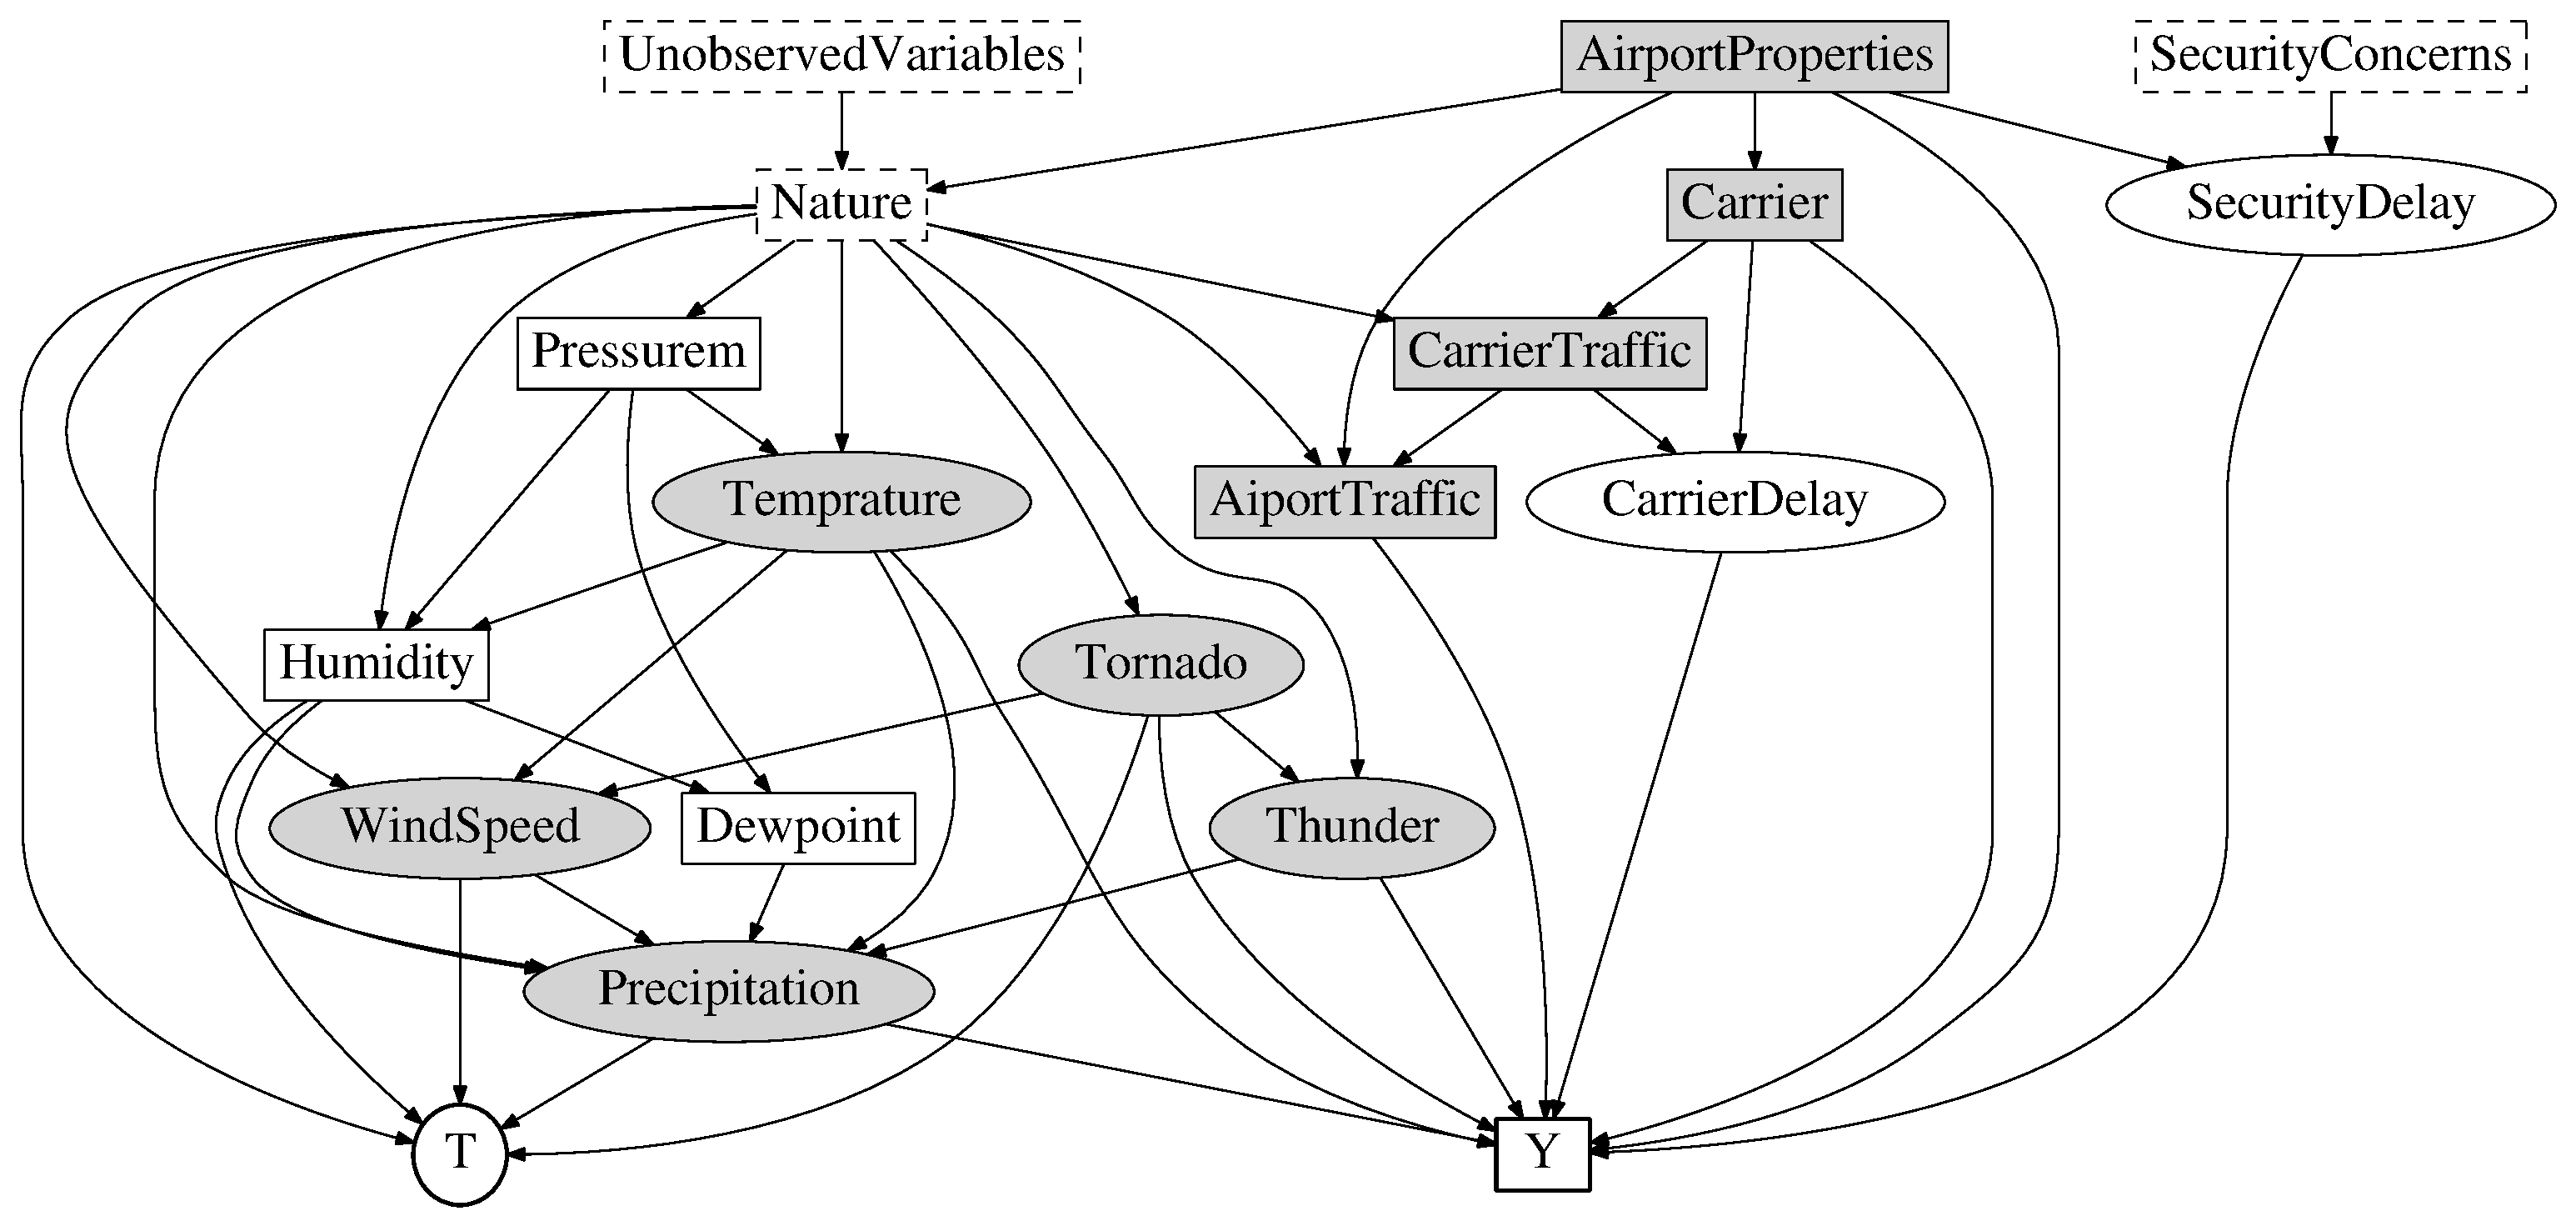
\includegraphics[width=1.1\linewidth]{Figures/dag.eps}
\caption{ {\bf \small A Causal Directed Acyclic Graph (CDAG)  demonstrating
    the assumptions necessary to estimate $\ate$ of the treatment
    T(LowVisibility) to the outcome Y(DepDelay).}  A CDAG shows how conditioning on observable covariates (X)
breaks the confounding causal relationships (e.g., T  $\leftarrow$ Precipitation
$\rightarrow$ Y) and allows the estimation of $\ate$. In other words, we assume that the treatment assignment $T$
and potential outcomes $Y=Y(z)$ for z=0,1 are unconfounded
by conditioning on the filled nodes which is a minimum cardinality set of {\em observed} variables that $d$-sperate the two. Attributes in boxes are from the flight data; Those in ovals are from the weather data; Those in dashed boxed are unobserved.}
\label{fig:dag}
\end{figure*}

\section{Experimental Results}
\label{sec:exp}

We have implemented the basic techniques in
Sec.~\ref{sec:BasicTechniques} and the optimizations in
Sec.~\ref{sec:OptimizationTechniques} in a system called \GSQL.  This
section, presents experiments that evaluate the feasibility and
efficacy of \GSQL.  We addressed the following questions.  What is the
end-to-end performance of \GSQL \ for causal inference in
observational data?  Does \GSQL \ support advanced methods for causal
inference and produce results with the same quality as statistical
software? How does \GSQL\ scale up with increasingly large data sets?
And how effective are the optimization techniques in \GSQL?

\vspace{-.2cm}

\subsection{Setup}
\label{sec:setup}

% \subsubsection{Data}
% \label{sec:data}

{\bf Data} The {\em flight dataset} we used was collected by the US
Department of Transportation (U.S. DOT) \cite{flightdata}. It contains
records of more than 90\% of US domestic flights of major airlines
from 1988 to the present. Table \ref{tab:attlist}(shown in Section
\ref{sec:introduction}) lists dataset attributes that are relevant to
our experiments.  We restrict our analysis to about 105M data entry
collected between 2000 and 2015.

The {\em weather dataset} was gathered using the weather underground
API \cite{Weatherdata}.  Its attributes are also presented in Table
\ref{tab:attlist}. In addition, we pre-computed two other attributes
AiportTraffic and CarrierTraffic. The former is the total number of
flights occur in the origin airport of a flight one hour prior to the
flight departure time, the latter is the same quantity restricted to
the flights from the same carrier.  We managed to acquire and clean
35M weather observations between 2000 and 2015. These datasets are
integrated by a spatio-temporal join.














% \subsubsection{Causal questions and covariate selection}
% \label{sec:def}

{\bf Causal questions and covariate selection} We explore the causal
effect of the following binary treatments on flight departure delays
and cancellation: LowVisibility (1 if Visim$<1$; 0 if Visim$>5$); \
Snow (1 iff Precipm$>0.3$ and Tempm$<0$); \ WindSpeed (1 if
Wspdm$>40$; 0 if Wspdm$<20$); \ and Thunder.  In each case, data items
where the attribute in question was in between the two bounds were
discarded.  For instance, for the treatment LowVisibility, we want to
assess the following counterfactual: {\em ``What would the flight
  departure delay have been, if visibility were fine, i.e., Visim$>5$,
  when visibility is actually low, i.e., Visim$<1$"}; for this
analysis, items where Visim$\in[1,5]$ were discarded.

% For each analysis, all flights not in the treated or control groups are discarded (for Snow and Thunder, all units are either treated or control).

\ignore{
We used the RNCM to estimate the $\ate$ of each treatment on flight departure delay and cancellation via the matching methods. Each flight
form a unit in the RNCM.} To ensure the SUTVA (cf. Section \ref{subsec:causalitystatistics}),  we considered the difference between the
actual delay and the late aircraft delay (if one exists) as the
outcome of interest. Therefore, we assumed that the potential delay of each flight did not depend on the treatment assignment
to the other flights namely, there was no interference between the units. \ignore{ To avoid multiple version of a treatment, we only considered extreme weather conditions as treatment. For instance, visibility in the range less than $1 km$ is considered as
treatment, assuming that any value of visibility in this range would have
a similar effect on flight departure delay.}






To obtain quality answers for each treatment, we used graphical models
to identify a minimum number of covariate attributes to ensure
unconfoundedness, because minimizing the number of covariates has been
shown to increase the precision of the matching estimators
\cite{de2011covariate}.  We used the tool provided by
\url{http://dagitty.net} to construct the causal DAG (CDAG) and select
the minimum number of covariates that separate the treatment assignments from  the potential outcomes.  The tool finds a minimal subset of variables $X$ that forms a
{\em $d$-separation}~\cite{PearlBook2000} of the treatment $T$ from
the effect $Y$ (meaning: all paths from $T$ to $Y$ go through some
variable in $X$).  For example, Figure \ref{fig:dag} shows the CDAG
for the treatment LowVisibility and the effect DepDelay: the set $X$
consists of the shaded nodes d-sperate the treatment assignment and the potential outcomes.

\ignore{

 shown in
to represent the causal relationships between LowVisibility, other features, and the
departure delay. \ignore{\footnote{}} Informally, CDAG is a carrier of independent assumptions provided that two
random variables (represented as nodes of the graph) are assumed to be independent iff there is no edge
between them. Further conditional independence can be extracted from  a CDAG by applying
the {\em d-separation} criterion \cite{PearlBook2000}. Informally, the point
of $d$-separation is that, if all paths in the CDAG leading from one random variable (say, $T_i$) to another (say, $Y_i$) are
blocked by a certain subset of variables (say, $X_i$), then $T_i$ and $Y_i$ are conditionally
independent given $X_i$. \ignore{For instance for LowVisibility we obtain that following minimal set of observed covariates:
$X$=\{AiportTraffic, CarrierTraffic, Precipitation, Temperature, Thunder, Tornado, Carrier, Windspeed\}.}
For instance, for LowVisibility, the filled nodes in Figure \ref{fig:dag}, represent the set of covariates that unconfound LowVisibility and DepDelay. For more details on covariate selection using CDAGs, we refer the reader to \cite{de2011covariate} and references therein.

}

{\bf Systems} The experiments were performed locally on a 64-bit OS X machine with
Intel Corei7 processor (16 GB RAM, 2.8 GHz).  \GSQL\
was deployed to Postgres version 9.5.  We compared \GSQL\ with R packages MatchIt
and CEM, version 2.4 and 1.1 respectively,  available from \cite{CRAN}.

\subsection{Results}








\subsubsection{End-to-End Performance} \label{sec:endtoend}

We estimated the causal effect of different weather types on flight departure delay and cancellation at five major US airports, that are among the ten airports with the worse weather-related delays according to \cite{weather},  namely: San Francisco (SFO) , John F. Kennedy (JFK), Newark Liberty (EWR), George Bush (IAH), and LaGuardia Airport (LGA).  The
flight and weather data associated with these airports consists of about 10M and 2M rows, respectively.

To this end, we estimated $\ate$  for each treatment associated to a weather type by performing CEM wrt. its identified covariates.  Continuous covariates were coarsened into equal width buckets, and categorical covariates were
matched by their exact values.

Figure \ref{fig:eteresult}(a) reports the running time of performing
CEM for each treatment: recall (Fig.~\ref{fig:cem}) that this involves
a group-by followed by an elimination of all groups that have no
treated, or no control unit.
\ignore{
 In this figure, the number of
treated and matched units for each treatment is represented as
labels. As depicted, CEM produced matched samples with reasonable
sizes.} Next, we evaluated the quality of the CEM, in Figure
\ref{fig:eteresult}(b), using a standard metric in the literature: the
{\em absolute weighted mean difference (AWMD)} of each continuous
covariate between the treated and control group:

{
\begin{align}
& \E_b[|\E[x_i | T=1, B(X)=b]-\E[x_i | T=0, B(X)=b]|] \label{eq:awmd}
\end{align}
}\noindent for each covariate attribute $x_i \in X$.  This is
a standard measure of imbalance, since in a perfectly balanced group
the difference is 0 (see Eq. \ref{eq:bs}). Note that in the case of CEM, we assume subclasses form the balancing scores.  We compared this
difference for the original value of the covarites  before and after CEM.  As shown, CEM substantially reduced
the covariates imbalance in the raw data: this graph shows the perils
of attempting to do causal inference naively, without performing CEM
or matching.  We also observed that CEM results in quite reasonable
matched sample size wrt. treatments ( more than 75\% of the treated
units are matched with the average rate of one treated to five control
units).


 \ignore{ we performed CEM in
  which the continuous covariates are simply coarsened by
  rounding. Figure \ref{fig:eteresult}(b,d) since data is pretty dense
  this simple coarsening strategy produced well-balanced matches with
  reasonable sizes. Figure \ref{fig:eteresult}(b,d) represents the
  estimation of $\ate$ for each treatments before and after CEM.}



\ignore{
. That is we measure the mean
difference of a covariate between the treated and control group within
each subclass and take the average of this quantity across all
subclasses.} \ignore{It is trivial that the matched sample is perfectly
  balanced on the categorical covariates such as Carrier.}


Next, Figure \ref{fig:eteresult}(c) shows the causal effect of weather
type on departure delay: it shows the estimated $\ate$ for each target
airport, normalized by the number of treated units to the total number
of units in each aiport.  Following common practice in causal
inference we estimated $\ate$ using Eq. \ref{eq:oatt} (thus assuming
that CEM produces perfectly balanced groups). The normalization lets
us compare the effects of different weather types in an individual
airport. In fact, $\ate$ reflects the potential causal effect of a
treatment to an outcome. For instance, IAH barely experiences snow,
but snow has a devastating effect on flight delay at this airport. The
results in Figure \ref{fig:eteresult}(c) are in line with those in
\cite{weather}, which reported the following major weather-related
causes of flight delay at the airports under the study:
snowstorms,thunderstorm and wind at EWR; thunderstorm and fog at IAH;
snowstorms and visibility at JFK; snowstorms at LGA; fog and low
clouds at SFO;


Figure \ref{fig:eteresult}(d) a similar causal effect of weather type
on a different outcome, namely Cancellation. Here, we leveraged the
fact that matching and subclassification do not depend on a particular
outcome variable, thus, a matched sample wrt. a treatment can be used
to estimate its causal effect of several outcomes.



\ignore{The credibility of the findings can be assessed by comparing the obtained $\ate$ for each treatment with the average difference
of weather delay and NAS delay between the treated and control group, we call
 this quantity {\em actual delay bound (ADB)}, as recorded in the flight dataset.
 ADB provides an upper bound for the actual causal effect of a weather type to departure delay.
As depicted in Figure \ref{fig:eteresult}(a), the estimated $\ate$ are always less than the ADB. In a similar way we measured
{\em actual cancellation bound (ACB)}, and compare it to the estimated effect of weather types on cancellation.}






\begin{figure*}
\hspace*{-0.7cm}\begin{subfigure}{0.62\linewidth}
\centering
%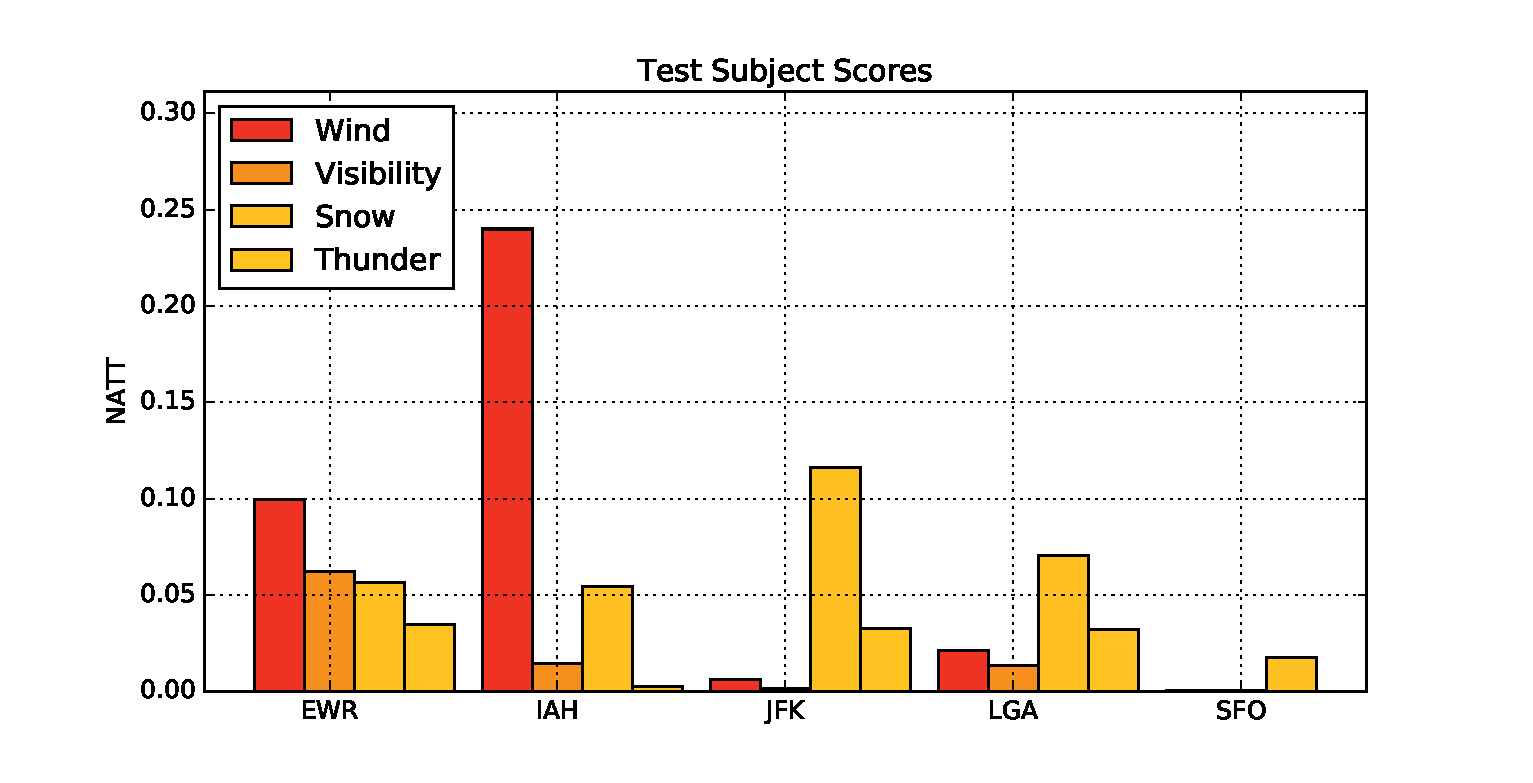
\includegraphics[width=.5\linewidth]{Figures/ATT(delay).eps}
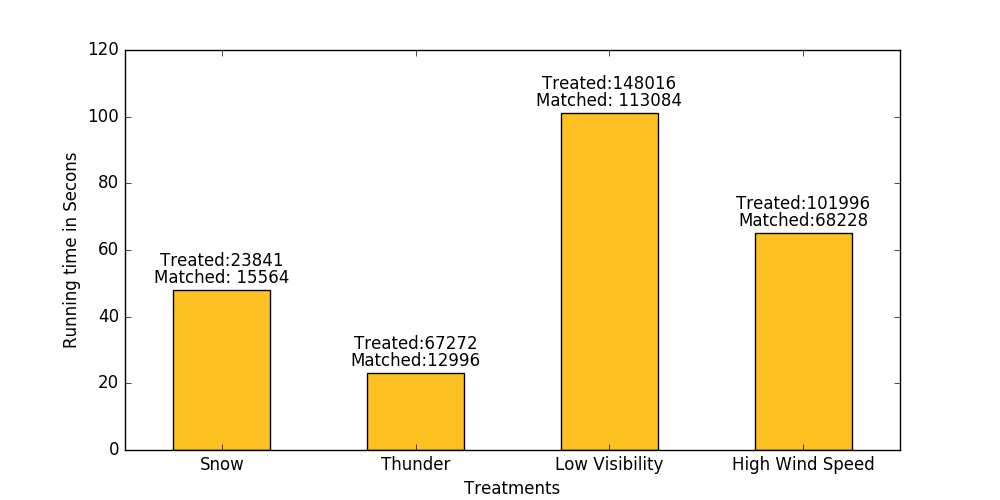
\includegraphics[height=5.5cm,width=\linewidth]{Figures/rtep1.png}
\caption{{Running Time of Matching.}}
\label{sfig:testa}
\end{subfigure}\hfill
\hspace*{-0.7cm}\begin{subfigure}{0.62\linewidth}
\centering
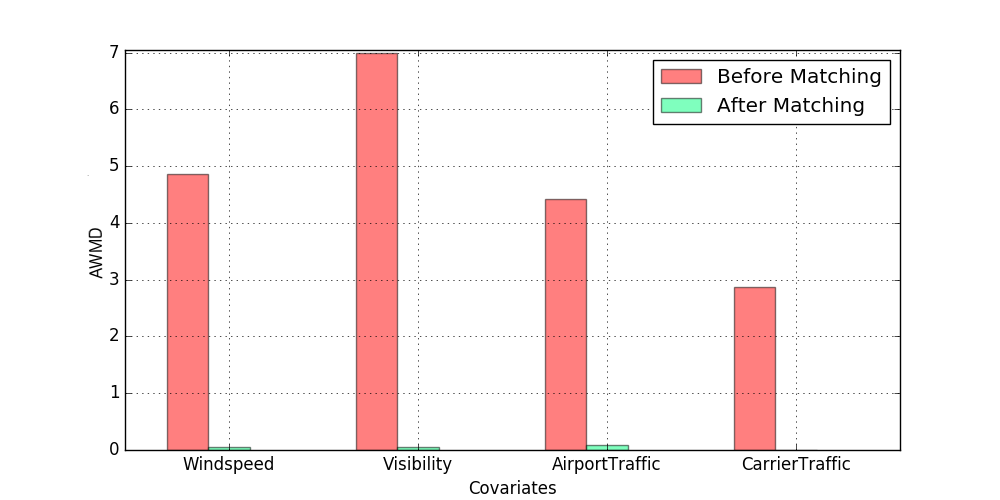
\includegraphics[height=5.5cm,width=\linewidth]{Figures/IR.png}
\caption{{Measuring Imbalance Reduction.}}
\label{sfig:testb}
\end{subfigure}\hfill

\hspace*{-0.7cm} \begin{subfigure}{0.62\linewidth}
\centering
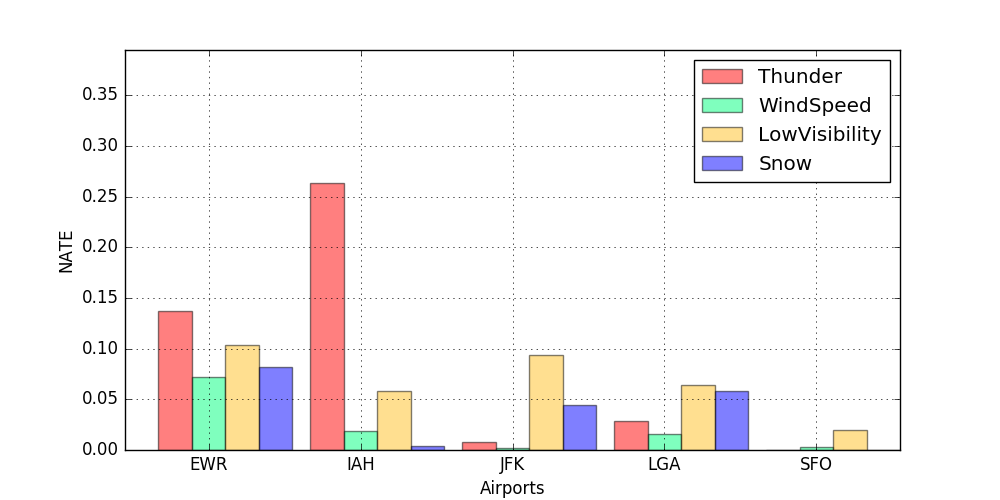
\includegraphics[height=5.5cm,width=\linewidth]{Figures/ATT(delay).png}
\caption{{Causal Effect of Weather Types on  Delay.}}
\label{sfig:testc}
\end{subfigure}\hfill
\hspace*{-0.7cm}\begin{subfigure}{0.62\linewidth}
\centering
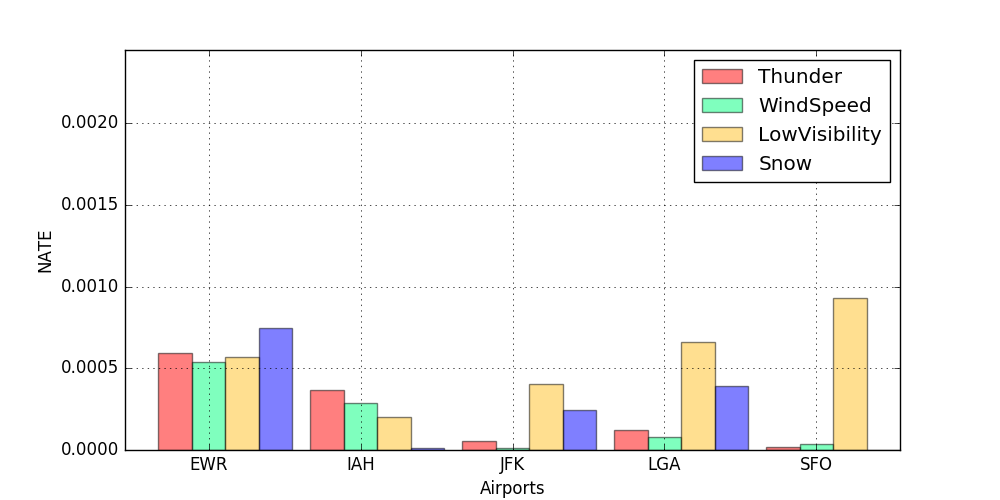
\includegraphics[height=5.5cm,width=\linewidth]{Figures/cancel.png}
\caption{{Causal Effect of Weather Types  on  Cancellation.}}
\label{sfig:testd}
\end{subfigure}\hfill

\caption{ \bf{Analysis of the causal effect of weather on flight delay and cancellation.}}
\label{fig:eteresult}
\end{figure*}




\vspace{-.3cm}
\subsubsection{Quality Comparisons with R}


% We compared the quality of the matching methods provided in \GSQL  \ with their
% counterpart methods in R. \ignore{More specifically, we compare exact matching,
% CEM, 1-1 NNMNR , 1-1 NNMWR and Subclassification
% based on propensity score with the similar methods
% provided in the MatchIt and CEM packages in R.}

The MatchIt and CEM packages in R are popular tools for conducting
causal inference today.  In this section we compare the quality of the
results returned by \GSQL\ with those returned by the R packages.  We
considered all types of matchings described in
Sec.~\ref{sec:BasicTechniques}: NN matching (both NNMNR and NNMWR),
and subclassification (by propensity score, CEM and exact matching(EM)).  Sine the R
packages do not scale to large datasets, we conducted these
experiments over a random sample of data used in Section
\ref{sec:endtoend}, which consists of around 210k rows. We evaluated
different matching methods for the treatment of Snow.


Table \ref{tbl:qc} compares the size of the matched sample and the
AWMD (Eq.\ref{eq:awmd}) obtained by \GSQL \ and R, for different
matching methods.  These results shows that \GSQL\ produced results
whose quality was at least as good as R.  Note that for NNMNR and
NNMWR, the caliper 0.001 is applied.   For subclassification all units with
propensity score less than 0.1 and more than 0.9 are discarded (this
is a common practice in causal inference). We observe that all
matching methods produce well-balance matched samples with reasonable
sizes. However, among these methods CEM works better both in terms of
the imbalance reduction and size of the matched sample.

The slight differences between
the results of NNM arose from a slight
difference between the propensity score distribution we obtained using logistic regression provided by MADlib inside Postgres. \ignore{ In addition, observe that subclassification in \GSQL \ did better than
it counterpart in R. This is because, }
%\cite{Hellerstein2012}

\ignore{
As represented in Table \ref{tbl:qc}, applying this caliper still provide us with a pretty reasonable sample size. Tables


This would increase the performance of
our NNM matching methods. We note that more sophisticated technics for performing NNM in SQL exists e.g., \cite{d}. However,
propensity score matching was not the main concern of our paper.}



\begin{table*}[t]
  \centering  \scriptsize
  \begin{tabular}{|c|c|c|c|c|c|c|c|} \hline
    & \multicolumn{3}{c|}{}   & \multicolumn{4}{c|}{\bf{Absolute Weighted Mean Difference (AWMD)}} \\ \hline
   \bf{Method} &  & \bf{Control} & \bf{Treated}  & \bf{Visibility} & \bf{WindSpeed}& \bf{AirportTraffic} & \bf{CarrierTraffic} \\ \hline
    & { \em Raw Data }
 & 214457 & 464 & 12.7529& 3.6363
&4.5394&2.9465 \\ \hline
 \raisebox{-.5\normalbaselineskip}[1pt][1pt]{\rotatebox[origin=c]{0}{\bf{NNMWR}}}&
R & 311 & 323
   &  0.0724
 & 0.8789
 &0.6935  &0.2724
 \\
 &\GSQL			& 296		&		312	&	 0.0692&	  0.5756&	0.6955	&0.8044
\\ \hline
 \raisebox{-.5\normalbaselineskip}[1pt][1pt]{\rotatebox[origin=c]{0}{\bf{NNMNR}}}&   R & 318
 & 318
 & 0.1006
 &1.0308
 & 0.3396&0.1352
\\
& \GSQL &	 291		&		291&0.0769&	0.7216& 	0.3195	& 0.5910
\\ \hline
 \raisebox{-.5\normalbaselineskip}[1pt][1pt]{\rotatebox[origin=c]{0}{\bf{Subclass.}}} &
 R &   1275 &255 & 2.5054
  & 1.4631
 & 1.6013&1.0022
\\
& \GSQL &1002 &
255& 0.0684&  1.0631&  0.1872&  0.0905
\\ \hline
 \raisebox{-.5\normalbaselineskip}[1pt][1pt]{\rotatebox[origin=c]{0}{\bf{EM}}} &      R & 8
 & 7
 & 0
 & 0
 & 0&0
 \\
 & \GSQL & 8
 & 7
 & 0
 & 0
 & 0&0
 \\ \hline
  \raisebox{-.5\normalbaselineskip}[1pt][1pt]{\rotatebox[origin=c]{0}{\bf{CEM}}} &     R &2284&
340&
0.2875 &  0.0542&   0.1135& 0.0905 \\
& \GSQL &2284&
340&
0.28755 &  0.0542&   0.1135& 0.0905 \\ \hline




    \end{tabular} \vspace{0.5cm}
    \caption{\bf{Quality Comparison between \GSQL \ and R.}}
  \label{tbl:qc}
\end{table*}



\vspace{-.25cm}
\subsubsection{Scalability Testing}
\label{sec:sct}
We compared the scalability of different matching methods in \GSQL \ and R. The experiment was carried out over
a random samples of data used in Section \ref{sec:endtoend} and for the treatment of Snow. Figure \ref{fig:perfresults}(a) compares NNM methods based on propensity score. We observe that NNM does not scale to large data. Note that, for the reasons mentioned in Section \ref{sec:nnm}, optimizing this method was not the aim of this paper. Figure \ref{fig:perfresults}(b)  compares CEM, EM and subclassification in \GSQL \ and R. Note that for CEM and NNMWR in \GSQL\, we respectively implemented the group-by and window function statement. As depicted,  \GSQL \ significantly outperforms R and scale to large data.



\begin{figure*}
\hspace*{-0.7cm}\begin{subfigure}{0.59\linewidth}
\centering
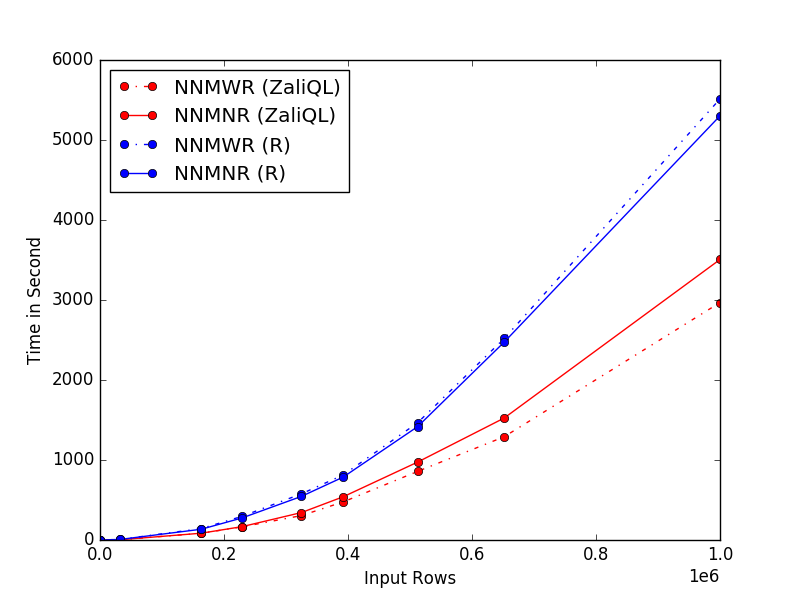
\includegraphics[height=5cm,width=1.02\linewidth]{Figures/NNM.png}
\caption{{Scalability Comparison (NNM).}}
\label{sfig:testaa}
\end{subfigure}\hfill
 \hspace*{-0.45cm}\begin{subfigure}{0.59\linewidth}
\centering
\vspace*{0.41cm} 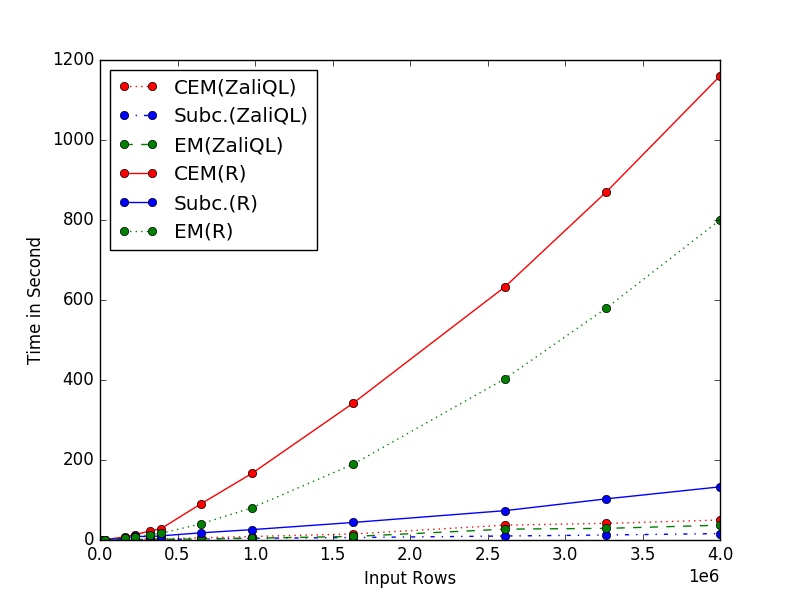
\includegraphics[height=5cm,width=1.02\linewidth]{Figures/exact.png}
\caption{{Scalability Comparison (CEM, EM and Subclas.).}}
\label{sfig:testbb}
\end{subfigure}\hfill

\hspace*{-0.7cm}\begin{subfigure}{0.59\linewidth}
\centering
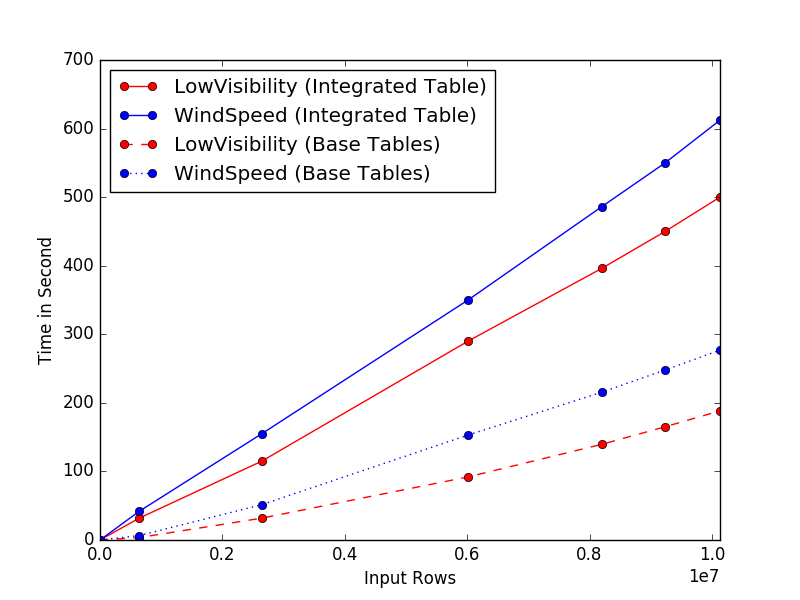
\includegraphics[height=5.5cm,width=1.02\linewidth]{Figures/opt1.png}
\caption{Efficacy of Pushing Matching.}
\label{sfig:testbc}
\end{subfigure}\hfill
\hspace*{-0.5cm}\begin{subfigure}{0.59\linewidth}
\centering \vspace{0.4cm}
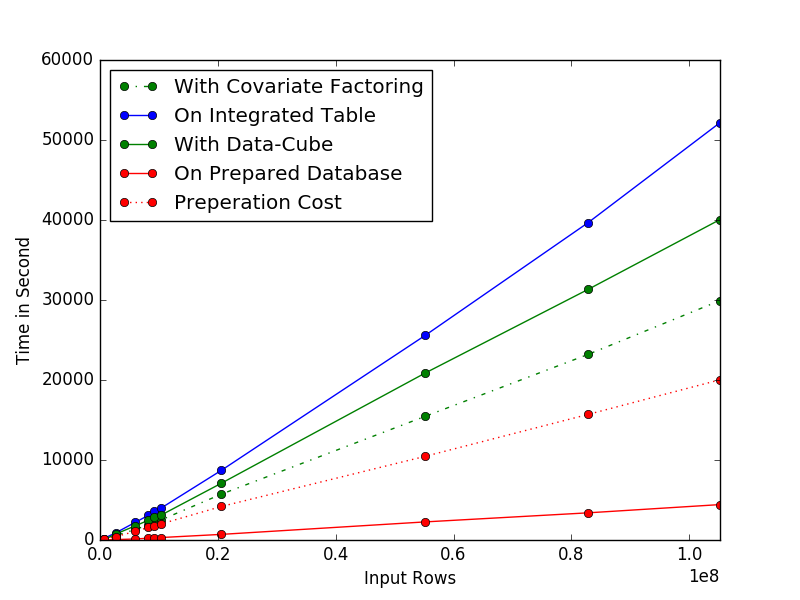
\includegraphics[height=5.5cm,width=1.02\linewidth]{Figures/push.png}
\caption{Efficacy of optimizations for multiple treatments.}
\label{sfig:testbd}
\end{subfigure}\hfill

\caption{\bf{Scalability and optimizations Evaluation.}}
\label{fig:perfresults}
\end{figure*}






\vspace{-.25cm}
\subsubsection{Efficacy of the Optimization Techniques}
\label{sec:opt}
We tested the effectiveness of the proposed optimization techniques (cf. Section \ref{sec:OptimizationTechniques}). Figure \ref{fig:perfresults}(c) compares the running time of performing CEM on
the integrated weather and flight tables with CEM on base tables (cf. Section \ref{sec:baserel})
for two treatment LowVisibility and WindSpeed.  The analysis was carried out on data used in Section \ref{sec:endtoend}. Note that the cost of integrating two tables is ignored.


For covariates factoring and data-cube optimizations, we compared the
total cost of performing matching on the treatments defined in Section
\ref{sec:setup}, plus the treatment obtained by conjunction of Snow and
WindSpeed, which we refer to as Snowstorm. This analysis was carried
on the entire integrated dataset. By applying Algorithm \ref{al:cf1},
the treatments are partitioned into two groups, namely $g_0$=\{Snow,
WindSpeed, Snowstorm\} and $g_2$=\{LowVisibility, Thunder\}.  Figure
\ref{fig:perfresults}(d) compares the total running time of matching
for each treatment after covariate factoring with the naive matching
procedure. Figure \ref{fig:perfresults}(d)  also shows the total cost of matching with and without using data-cubes.
 In addition, it represents the total cost of matching on the prepared database, according to Algorithm \ref{alg:dp}, and the cost of database preparation. As depicted,  matching on the prepared database
reduce the over cost of matching by an order of magnitude.  \ignore{Observe that the total cost of performing matching on the prepared database plus the cost of preparation is less than matching using only data-cube and covariates factoring. \ignore{Therefore, Algorithm \ref{alg:dp} can also be applied to the setting that }}


\ignore{
{\em Matching on bases tables:} Figure \ref{fig:perfresults}(b) compares the running time of performing CEM on
the pre-integrated weather and flight tables with CEM on base tables (cf. Section \ref{sec:baserel}). The comparison
is made on different sample sizes. Note that the cost
of joining two tables is ignored.


{\em Factorization:} we evaluate the factorization technique to  optimize the overall cost of performing matching
for $T_1$ \ldots $T_4$. To this end first we apply the Algorithm
and obtained the following treatment partitions.  [...] Figure \ref{fig:perfresults}(c)


{\em Data-cubes:} We used the data-cube technique to optimize the overall cost of performing matching
for $T_1$, $T_2$, $T_3$ and any treatments
that can be defined by conjunction of these treatments e.g., we can define $T_{12}$ as 1 if $T_1$ and $T_2$
are 1 and 0 otherwise. Therefore, we have seven treatments in total. Figure  \ref{fig:perfresults}(d) compares the over cost of performing matching for these seven treatments independently and computing them based on the ton-down approach using
data-cubes.
}





